\documentclass[border=4pt]{standalone}
\usepackage{graphicx,amsmath,amssymb,amsfonts,xcolor}
\usepackage{tikz}
\usepackage{pgfplots}
\usepackage{scalerel}
\usetikzlibrary{positioning, decorations.pathreplacing, calligraphy, calc, shapes.geometric, intersections, arrows}
\usepgfplotslibrary{fillbetween}
\pgfplotsset{compat=1.18}

\newcommand{\fmri}{functional magnetic resonance imaging}
\newcommand{\FMRI}{Functional magnetic resonance imaging}
\newcommand{\fmriabbrv}{fMRI}
\newcommand{\eeg}{electroencephalography}
\newcommand{\EEG}{Electroencephalography}
\newcommand{\eegabbrv}{EEG}
\newcommand{\verify}[1]{\textcolor{red}{[VERIFY: #1]}}

\setlength{\textwidth}{372pt}
\begin{document}
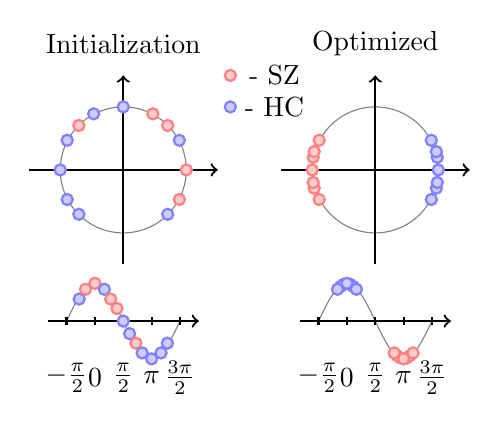
\begin{tikzpicture}
        [scale=0.8,
        inner sep=0.5mm,
        pd/.style={circle,draw=red!50,fill=red!20,thick},
        hc/.style={circle,draw=blue!50,fill=blue!20,thick}]
        
        %draw unit circle
        \node (uni_circle1) at (0,0) {};
        \draw[black!50, thin] ($(uni_circle1)$) circle [radius=1];
        \draw[black, thick, ->] ($(uni_circle1)+(-1.5,0)$) -- ($(uni_circle1)+(1.5,0)$);%xaxis
        \draw[black, thick, ->] ($(uni_circle1)+(0,-1.5)$) -- ($(uni_circle1)+(0,1.5)$);%yaxis
        
        \node (ind1) at ($(uni_circle1)+(1,0)$) [pd] {};
        \node (ind2) at ($(uni_circle1)+(0,1)$) [hc] {};
        \node (ind1) at ($(uni_circle1)+(-0.705,0.705)$) [pd] {};
        \node (ind1) at ($(uni_circle1)+(0.705,0.705)$) [pd] {};
        \node (ind1) at ($(uni_circle1)+(0.47,0.89)$) [pd] {};
        \node (ind2) at ($(uni_circle1)+(-1,0)$) [hc] {};
        \node (ind2) at ($(uni_circle1)+(-0.89,-0.47)$) [hc] {};
        \node (ind2) at ($(uni_circle1)+(-0.705,-0.705)$) [hc] {};
        \node (ind2) at ($(uni_circle1)+(0.89,0.47)$) [hc] {};
        \node (ind2) at ($(uni_circle1)+(-0.89,0.47)$) [hc] {};
        \node (ind2) at ($(uni_circle1)+(-0.47,0.89)$) [hc] {};
        \node (ind2) at ($(uni_circle1)+(0.89,-0.47)$) [pd] {};
        \node (ind2) at ($(uni_circle1)+(0.705,-0.705)$) [hc] {};
        
        
        \node (legend) at ($(uni_circle1)+(1.7,1)$) {};
        \node at ($(legend)+(0.7,0.5)$) {- SZ};
        \node at ($(legend)+(0.7,0)$) {- HC};
        \node at ($(legend)+(0,0.5)$) [pd] {};
        \node at ($(legend)+(0,0)$) [hc] {};
        
        %draw unit circle
        \node (uni_circle2) at ($(uni_circle1)+(4,0)$) {};
        \draw[black!50, thin] ($(uni_circle2)$) circle [radius=1];
        \draw[black, thick, ->] ($(uni_circle2)+(-1.5,0)$) -- ($(uni_circle2)+(1.5,0)$);%xaxis
        \draw[black, thick, ->] ($(uni_circle2)+(0,-1.5)$) -- ($(uni_circle2)+(0,1.5)$);%yaxis
        
        
        %individuals
        \node (ind1) at ($(uni_circle2)+(-1,0)$) [pd] {};
        \node (ind1) at ($(uni_circle2)+(-0.89,0.47)$) [pd] {};
        \node (ind1) at ($(uni_circle2)+(-0.985,0.2)$) [pd] {};
        \node (ind1) at ($(uni_circle2)+(-0.97,0.29)$) [pd] {};
        \node (ind1) at ($(uni_circle2)+(-0.89,-0.47)$) [pd] {};
        \node (ind1) at ($(uni_circle2)+(-0.97,-0.29)$) [pd] {};
        \node (ind1) at ($(uni_circle2)+(-0.985,-0.2)$) [pd] {};
        
        \node (ind2) at ($(uni_circle2)+(1,0)$) [hc] {};
        \node (ind1) at ($(uni_circle2)+(0.89,0.47)$) [hc] {};
        \node (ind1) at ($(uni_circle2)+(0.985,0.2)$) [hc] {};
        \node (ind1) at ($(uni_circle2)+(0.97,0.29)$) [hc] {};
        \node (ind1) at ($(uni_circle2)+(0.89,-0.47)$) [hc] {};
        \node (ind1) at ($(uni_circle2)+(0.97,-0.29)$) [hc] {};
        \node (ind1) at ($(uni_circle2)+(0.985,-0.2)$) [hc] {};
        
        
        
        \node (sinusoid1) at ($(uni_circle1)+(0,-2.7)$) {};
        \draw[black, thick, ->] ($(sinusoid1)+(-1.2,0.3)$) -- ($(sinusoid1)+(1.2,0.3)$);%xaxis
        \draw[thin, black!50] ($(sinusoid1)+(0.9,0.3)$) sin ($(sinusoid1)+(0.45,-0.3)$);
        \draw[thin, black!50] ($(sinusoid1)+(0.45,-0.3)$) cos ($(sinusoid1)+(0.,0.3)$);
        \draw[thin, black!50] ($(sinusoid1)+(0.,0.3)$) sin ($(sinusoid1)+(-0.45,0.9)$);
        \draw[thin, black!50] ($(sinusoid1)+(-0.45,0.9)$) cos ($(sinusoid1)+(-0.9,0.3)$);
        
        \draw[black, thick] ($(sinusoid1)+(-0.9,0.36)$) -- ($(sinusoid1)+(-0.9,0.24)$);
        
        \draw[black, thick] ($(sinusoid1)+(-0.45,0.36)$) -- ($(sinusoid1)+(-0.45,0.24)$);
        \draw[black, thick] ($(sinusoid1)+(0.,0.36)$) -- ($(sinusoid1)+(0.,0.24)$);
        \draw[black, thick] ($(sinusoid1)+(0.45,0.36)$) -- ($(sinusoid1)+(0.45,0.24)$);
        \draw[black, thick] ($(sinusoid1)+(0.9,0.36)$) -- ($(sinusoid1)+(0.9,0.24)$);
        
        \node at ($(sinusoid1)+(-0.9,-0.6)$) {$-\frac{\pi}{2}$};
        \node at ($(sinusoid1)+(-0.45,-0.6)$) {$0$};
        \node at ($(sinusoid1)+(0.,-0.6)$) {$\frac{\pi}{2}$};
        \node at ($(sinusoid1)+(0.45,-0.6)$) {$\pi$};
        \node at ($(sinusoid1)+(0.9,-0.6)$) {$\frac{3\pi}{2}$};
        
        \node (ind1) at ($(sinusoid1)+(-0.7,0.65)$) [hc] {};
        \node (ind1) at ($(sinusoid1)+(-0.6,0.805)$) [pd] {};
        \node (ind1) at ($(sinusoid1)+(-0.45,0.9)$) [pd] {};
        \node (ind1) at ($(sinusoid1)+(-0.3,0.805)$) [hc] {};
        \node (ind1) at ($(sinusoid1)+(-0.2,0.65)$) [pd] {};
        \node (ind1) at ($(sinusoid1)+(-0.1,0.5)$) [pd] {};
        \node (ind1) at ($(sinusoid1)+(0.,0.3)$) [hc] {};
        \node (ind1) at ($(sinusoid1)+(0.1,0.1)$) [hc] {};
        \node (ind1) at ($(sinusoid1)+(0.2,-0.05)$) [pd] {};
        \node (ind1) at ($(sinusoid1)+(0.3,-0.205)$) [hc] {};
        \node (ind1) at ($(sinusoid1)+(0.45,-0.3)$) [hc] {};
        \node (ind1) at ($(sinusoid1)+(0.6,-0.205)$) [hc] {};
        \node (ind1) at ($(sinusoid1)+(0.7,-0.05)$) [hc] {};
        
        \node (sinusoid2) at ($(uni_circle2)+(0,-2.7)$) {};
        \draw[black, thick, ->] ($(sinusoid2)+(-1.2,0.3)$) -- ($(sinusoid2)+(1.2,0.3)$);%xaxis
        \draw[thin, black!50] ($(sinusoid2)+(0.9,0.3)$) sin ($(sinusoid2)+(0.45,-0.3)$);
        \draw[thin, black!50] ($(sinusoid2)+(0.45,-0.3)$) cos ($(sinusoid2)+(0.,0.3)$);
        \draw[thin, black!50] ($(sinusoid2)+(0.,0.3)$) sin ($(sinusoid2)+(-0.45,0.9)$);
        \draw[thin, black!50] ($(sinusoid2)+(-0.45,0.9)$) cos ($(sinusoid2)+(-0.9,0.3)$);
        
        \draw[black, thick] ($(sinusoid2)+(-0.9,0.36)$) -- ($(sinusoid2)+(-0.9,0.24)$);
        
        \draw[black, thick] ($(sinusoid2)+(-0.45,0.36)$) -- ($(sinusoid2)+(-0.45,0.24)$);
        \draw[black, thick] ($(sinusoid2)+(0.,0.36)$) -- ($(sinusoid2)+(0.,0.24)$);
        \draw[black, thick] ($(sinusoid2)+(0.45,0.36)$) -- ($(sinusoid2)+(0.45,0.24)$);
        \draw[black, thick] ($(sinusoid2)+(0.9,0.36)$) -- ($(sinusoid2)+(0.9,0.24)$);
        
        \node at ($(sinusoid2)+(-0.9,-0.6)$) {$-\frac{\pi}{2}$};
        \node at ($(sinusoid2)+(-0.45,-0.6)$) {$0$};
        \node at ($(sinusoid2)+(0.,-0.6)$) {$\frac{\pi}{2}$};
        \node at ($(sinusoid2)+(0.45,-0.6)$) {$\pi$};
        \node at ($(sinusoid2)+(0.9,-0.6)$) {$\frac{3\pi}{2}$};
        
        
        \node (ind1) at ($(sinusoid2)+(-0.5,0.885)$) [hc] {};
        \node (ind1) at ($(sinusoid2)+(-0.55,0.85)$) [hc] {};
        \node (ind1) at ($(sinusoid2)+(-0.6,0.805)$) [hc] {};
        \node (ind1) at ($(sinusoid2)+(-0.4,0.885)$) [hc] {};
        \node (ind1) at ($(sinusoid2)+(-0.35,0.85)$) [hc] {};
        \node (ind1) at ($(sinusoid2)+(-0.3,0.805)$) [hc] {};
        \node (ind1) at ($(sinusoid2)+(-0.45,0.9)$) [hc] {};
        
        
        \node (ind1) at ($(sinusoid2)+(0.5,-0.285)$) [pd] {};
        \node (ind1) at ($(sinusoid2)+(0.55,-0.25)$) [pd] {};
        \node (ind1) at ($(sinusoid2)+(0.6,-0.205)$) [pd] {};
        \node (ind1) at ($(sinusoid2)+(0.4,-0.285)$) [pd] {};
        \node (ind1) at ($(sinusoid2)+(0.35,-0.25)$) [pd] {};
        \node (ind1) at ($(sinusoid2)+(0.3,-0.205)$) [pd] {};
        \node (ind1) at ($(sinusoid2)+(0.45,-0.3)$) [pd] {};
        
        \node (title1) at ($(uni_circle1)+(0,2)$) {Initialization};
        \node (title2) at ($(uni_circle2)+(0,2)$) {Optimized};
        
        %\node (stats1) at ($(uni_circle1)+(0,-4)$) {$\mathbb{E}[f_x(x)]=\frac{\pi}{2}, \mbox{Var}[f_x(x)]=\frac{\pi}{2}$};
        %\node (stats2) at ($(uni_circle2)+(0,-4)$) {$\mathbb{E}[f_x(x)]=\frac{\pi}{2}, \mbox{Var}[f_x(x)]=\frac{\pi}{2}$};
        
    \end{tikzpicture}
\end{document}
